\newcommand{\psd}[1]{{\small\sffamily{\color{blue!60}#1}}}

In this section we present a 3D PSD simulation of a clamped bar which
his being loaded in vertical direction at the non-clamped end. This
simulation is like the one presented in previous tutorials, however in
3D. The material properties are same as before, and at the non-clamped
end traction \(t_y=-10^9\) units. The 3D bar is \(1\times1\times5\)
m\(^3\).

Here is how PSD simulation of this case can be performed.

\textbf{Step 1: Preprocessing}

For ``PSD setup'' go to any folder, launch the terminal there and run
the following command.

\begin{lstlisting}[style=BashInputStyle]
PSD_PreProcess  -problem linear-elasticity -dimension 3 -dirichletconditions 1 -tractionconditions 1 -postprocess u
\end{lstlisting}

\% the comandline flag \psd{ -dirichletconditions 1} notifies to PSD
that there is one Dirichlet border ---the clamped end of the bar--- in
this simulation; \psd{ -dimension 3} means the simulation is 3D. And the
flag \psd{ -tractionconditions 1} notifies to PSD that there is one
traction border ---the right end of the bar--- in this simulation. To
provide Dirichlet conditions of the clamped end (\(u_x=0,u_y=0,u_z=0\))
in \psd{ ControlParameters.edp} set \psd{ Dbc0On 1}, \psd{ Dbc0Ux 0.},
\psd{ Dbc0Uy 0.}, and \psd{ Dbc0Uz 0.}, where 1 being the surface mesh
label of the clamped end. To add the traction boundary condition set
\psd{ Tbc0On 2} and \psd{ Tbc0Ty -1.e9}, here the mesh label number of
the right end is 2. For this end
\(\mathbf t=[t_x,t_y,t_z]=[0.,10^9,0.]\), hence in
\psd{ ControlParameters.edp} we only use \psd{ Tbc0Ty -1.e9}.

\textbf{Step 2: Solving}

Let us now use 4 cores to solve this problem. To do so enter the
following command:

\begin{lstlisting}[style=BashInputStyle]
PSD_Solve -np 4 Main.edp
\end{lstlisting}

\% Notice, that this is the exact same command used in solving the
previous bar problems from other sections.

\textbf{Step 3: Postprocessing}

Launch ParaView and have a look at the \psd{ .pvd} file in the
\psd{ PSD/Solver/VTUs\_DATE\_TIME} folder.

\begin{figure}[htbp]
    \centering
    \begin{minipage}[t][2cm][t]{0.38\textwidth}
    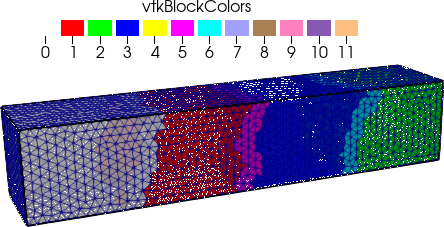
\includegraphics[align=b,width=1\textwidth]{./Images/3d-bar-clamped-ends.png}
    \end{minipage}\hspace{.1\textwidth}
    \begin{minipage}[t][2cm][t]{0.4\textwidth}
    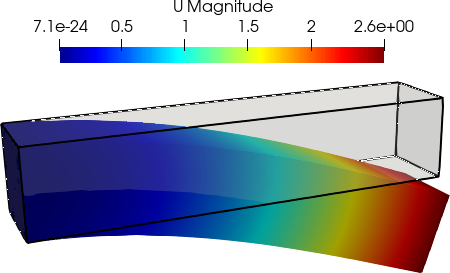
\includegraphics[align=b,width=1\textwidth]{./Images/3d-bar-clamped-pulled-partioned.png}
    \end{minipage}
    \caption{3D bar results. Partitioned mesh (left) and 0.5X warped displacement field (right).}
    \label{fig:3Dpart}
\end{figure}

In\textasciitilde{}\cref{fig:3Dpart} there are four subdomais in the
partitioned mesh since four cores were used.
